\documentclass[12pt, a4paper]{extarticle}
\usepackage{GOST}
\usepackage{array}
\usepackage{verbatim}
\usepackage[detect-all]{siunitx}
\usepackage{amsmath}
\usepackage{amssymb}
\usepackage[utf8]{inputenc}
\usepackage{hyperref}
\usepackage{tempora}

\makeatletter
\renewcommand\@biblabel[1]{#1.}
\makeatother

\usepackage{listings}
\lstset{ 
	language=Prolog,
	basicstyle = \ttfamily\color{blue},
	moredelim = [s][\color{black}]{(}{)},
	tabsize=4,
	literate =
	{:-}{{\textcolor{black}{:-}}}2
	{,}{{\textcolor{black}{,}}}1
	{.}{{\textcolor{black}{.}}}1
}



\begin{document}
	
\begin{table}[ht]
	\centering
	\begin{tabular}{|c|p{400pt}|} 
		\hline
		\begin{tabular}[c]{@{}c@{}} 
\includegraphics[scale=1]{source/b_logo.jpg} \\\end{tabular} &
		\footnotesize\begin{tabular}[c]{@{}c@{}}\textbf{Министерство~науки~и~высшего~образования~Российской~Федерации}\\\textbf{Федеральное~государственное~бюджетное~образовательное~учреждение}\\\textbf{~высшего~образования}\\\textbf{«Московский~государственный~технический~университет}\\\textbf{имени~Н.Э.~Баумана}\\\textbf{(национальный~исследовательский~университет)»}\\\textbf{(МГТУ~им.~Н.Э.~Баумана)}\\\end{tabular}  \\
		\hline
	\end{tabular}
\end{table}
\noindent\rule{\textwidth}{4pt}
\noindent\rule[14pt]{\textwidth}{1pt}
\hfill 
\noindent
\makebox{ФАКУЛЬТЕТ~}%
\makebox[\textwidth][l]{\underline{~«Информатика и системы управления»~~~~~~~~~~~~~~~~~~~~~~~~~~~~~~~~~}}%
\\
\noindent
\makebox{КАФЕДРА~}%
\makebox[\textwidth][l]{\underline{~«Программное обеспечение ЭВМ и информационные технологии»~}}%
\\

\begin{center}
	\vspace{1.5cm}
	{\bf\huge Отчёт\par}
	{\bf\Large по лабораторной работе № 15\par}
	\vspace{0.7cm}
\end{center}


\noindent
\makebox{\large{\bf Название:}~~~}
\makebox[\textwidth][l]{\large\underline{~Структура программы на Prolog и ее реализация~}}\\

\noindent
\makebox{\large{\bf Дисциплина:}~~~}
\makebox[\textwidth][l]{\large\underline{~Функциональное и логическое программирование~}}\\

\vspace{1.5cm}
\noindent
\begin{tabular}{l c c c c c}
	Студент      & ~ИУ7-65Б~               & \hspace{2.5cm} & \hspace{2cm}                 & &  Д.В. Сусликов \\\cline{2-2}\cline{4-4} \cline{6-6} 
	\hspace{3cm} & {\footnotesize(Группа)} &                & {\footnotesize(Подпись, дата)} & & {\footnotesize(И.О. Фамилия)}
\end{tabular}

\noindent
\begin{tabular}{l c c c c}
	Преподаватель & \hspace{5cm}   & \hspace{2cm}                 & & ~~~~~~Н.Б. Толпинская~~~~~~\\\cline{3-3} \cline{5-5} 
	\hspace{3cm}  &                & {\footnotesize(Подпись, дата)} & & {\footnotesize(И.О. Фамилия)}
\end{tabular}

\vspace{0.6cm}
\begin{center}	
	\vfill
	\large \textit {Москва, 2021}
\end{center}

\thispagestyle {empty}
\pagebreak

\clearpage


\textbf{Цель работы} - изучить структуру, особенности и принципы оформления программы, и способ выполнения программы на Prolog

\textbf{Задание}
	Создать базу знаний «Собственники», дополнив базу знаний, хранящую знания (лаб. 13):
	\begin{itemize}
		\item <<Телефонный справочник>>: Фамилия, №тел, Адрес – структура (Город, Улица, №дома, №кв),
		\item <<Автомобили>>: Фамилия\_владельца, Марка, Цвет, Стоимость, и др.,
		\item <<Вкладчики банков>>: Фамилия, Банк, счет, сумма, др.,
	\end{itemize}
	знаниями о дополнительной собственности владельца. Преобразовать знания об автомобиле к форме знаний о собственности.
	Вид собственности (кроме автомобиля):
	\begin{itemize}
		\item Строение, стоимость и другие его характеристики;
		\item Участок, стоимость и другие его характеристики;
		\item Водный\_транспорт, стоимость и другие его характеристики.
	\end{itemize}
	
	Описать  и использовать вариантный домен: Собственность. Владелец может иметь, но только один объект каждого вида собственности (это касается и автомобиля), или не иметь некоторых видов собственности. 
	
	\hfill
	
	Используя конъюнктивное правило и разные формы задания одного вопроса, обеспечить возможность поиска:
	\begin{enumerate}
		\item Названий всех объектов собственности заданного субъекта,
		\item Названий и стоимости всех объектов собственности заданного субъекта,
		\item Разработать правило, позволяющее найти суммарную стоимость всех объектов собственности заданного субъекта.
	\end{enumerate}
	
	\hfill
	
	Для 2-го пункт и одной фамилии составить таблицу, отражающую конкретный порядок работы системы, с объяснениями порядка работы и особенностей использования доменов (указать конкретные Т1 и Т2 и полную подстановку на каждом шаге)
	
	
	\newpage
	
	\textbf{Листинг:}
	
	\begin{lstlisting}
	domains
		number, surname, city, street, brand, color, bank = symbol.
		building_num, room_num, price, bill, summa, square, cost = integer.
		address = address(city, street, building_num, room_num).
	
		property = 	  car(brand, color, cost);
							building(cost, street, building_num);
							ground(cost, square);
							water_transport(cost, color).
	
	predicates
		phonebook(surname, number, address).
		depositor(surname, bank, bill, summa).
	
		own(surname, property).
		own_by_name(surname, symbol).
		own_price_by_name(surname, symbol, cost).
		
	clauses
		phonebook("Surname1","11111", address("City1", "St.1", 1, 17)).
		phonebook("Surname2","22222", address("City2", "St.2", 2, 18)).
		phonebook("Surname3","33333", address("City1", "St.1", 4, 28)).
		phonebook("Surname4","11111", address("City3", "St.4", 4, 24)).
		
		depositor("Surname1", "Bank1", 3221, 1200).
		depositor("Surname1", "Bank2", 1233, 4000).
		depositor("Surname2", "Bank2", 4356, 2000).
		
		own("Surname1", car("Brand1", "Red", 12345)).
		own("Surname1", ground(4321, 1000)).
		own("Surname1", water_transport(22233, "Black")).
		own("Surname2", car("Brand2", "Blue", 30000)).
		own("Surname2", building(49000, "St.1", 13)).
		own("Surname3", car("Brand3", "Grey", 32213)).
		own("Surname3", ground(4567, 1100)).
		
		own_by_name(Name, Property):- own(Name, car(_, _, _)), Property = "Car".
		own_by_name(Name, Property):- own(Name, building(_, _, _)), Property = 	"Building".
		own_by_name(Name, Property):- own(Name, ground(_, _)), Property = "Ground".
		own_by_name(Name, Property):- own(Name, water_transport(_, _)), Property = "Water Transport".
		
		own_price_by_name(Name, Property, Price):- own(Name, car(_, _, Price)), Property = "Car".
		own_price_by_name(Name, Property, Price):- own(Name, building(Price, _, _)), Property = "Building".
		own_price_by_name(Name, Property, Price):- own(Name, ground(Price, _)), Property = "Ground".
		own_price_by_name(Name, Property, Price):- own(Name, water_transport(Price, _)), Property = "Water Transport".
	
	goal
		% Task1.
		%own_by_name("Surname1", Property).
		%own_by_name("Surname3", Property).
		%own_by_name("Surname4", Property).
		
		% Task2.	
		%own_price_by_name("Surname1", Property, Price).
		%own_price_by_name("Surname3", Property, Price).
		%own_price_by_name("Surname4", Property, Price).
	
\end{lstlisting}
\newpage

\textbf{1) Названия всех объектов собственности заданного субъекта.}\par
\begin{figure}[h!]	
	\center{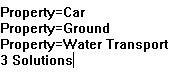
\includegraphics{source/1.1.png} \\ Пример 1.1}	
\end{figure}\par

\begin{figure}[h!]	
	\center{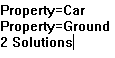
\includegraphics{source/1.2.png} \\ Пример 1.2}	
\end{figure}\par

\begin{figure}[h!]	
	\center{
\includegraphics{source/no_sol.png} \\ Пример 1.3}	
\end{figure}\par

\textbf{2) Названия и стоимости всех объектов собственности заданного субъекта.}\par

\begin{figure}[h!]	
	\center{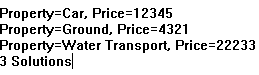
\includegraphics{source/2.1.png} \\ Пример 2.1}	
\end{figure}\par

\begin{figure}[h!]	
	\center{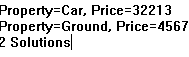
\includegraphics{source/2.2.png} \\ Пример 2.2}	
\end{figure}\par

\begin{figure}[h!]	
	\center{
\includegraphics{source/no_sol.png} \\ Пример 2.3}	
\end{figure}\par

\newpage
\textbf{Таблица}\par
own\_price\_by\_name("Surname1", Property, Price).\par
\begin{table}[h!]
	\begin{tabular}{|l|l|l|}
		\hline
		Шаг & \begin{tabular}[c]{@{}l@{}}Сравнимые термы; результаты; \\ подстановка, если есть\end{tabular}                                                                                                                                                    & Дальнейшие действия                                                                                                                                                                                                                                 \\ \hline
		1   & \begin{tabular}[c]{@{}l@{}}own\_price\_by\_name("Surname1" , Property, Price)\\ phonebook(...)\\ \\ Неудача. Не унифицируемы.\end{tabular}                                                                                                        & \begin{tabular}[c]{@{}l@{}}Переход к следующему\\ заголовку БЗ\end{tabular}                                                                                                                                                                         \\ \hline
		& ...                                                                                                                                                                                                                                               &                                                                                                                                                                                                                                                     \\ \hline
		2  & \begin{tabular}[c]{@{}l@{}}own\_price\_by\_name("Surname1", Property, Price)\\ own\_price\_by\_name(Name, Property, Price)\\ \\ Успех. Унифицируемы.\\ \\ Подстановка: \{Name = "Surname1" , \\ Property = Property, Price = Price\}\end{tabular} & \begin{tabular}[c]{@{}l@{}}Смена состояния резольвенты.\\ Новое состояние резольвенты:\\ own("Surname1" , car(\_, \_, Price)), \\ Property = "Car".\end{tabular}                                                                                    \\ \hline
		3  & \begin{tabular}[c]{@{}l@{}}own("Surname1" , car(\_, \_, Price))\\ phonebook(...)\\ \\ Неудача. Не унифицируемы.\end{tabular}                                                                                                                      & \begin{tabular}[c]{@{}l@{}}Переход к следующему\\ заголовку БЗ\end{tabular}                                                                                                                                                                         \\ \hline
		& ...                                                                                                                                                                                                                                               &                                                                                                                                                                                                                                                     \\ \hline
		4  & \begin{tabular}[c]{@{}l@{}}own("Surname1" , car(\_, \_, Price))\\ own("Surname1" , car("Brand1" , "Red" , 12345))\\ \\ Успех. Унифицируемы.\\ \\ Подстановка: \{"Surname1" = "Surname1" , \\ Price = 12345\}\end{tabular}                         & \begin{tabular}[c]{@{}l@{}}Смена состояния резольвенты.\\ Новое состояние резольвенты:\\ Property = "Car"\end{tabular}                                                                                                                              \\ \hline
		5  &                                                                                                                                                                                                                                                   & \begin{tabular}[c]{@{}l@{}}Смена состояния резольвенты.\\ Новое состояние резольвенты:\\ Пустая\\  Вывод:\\ Property=Car, Price=12345 \\ Новое состояние резольвенты:\\ own("Surname1" , car(\_, \_, Price)), \\ Property = "Car".\end{tabular} \\ \hline

	\end{tabular}
\end{table}

\begin{table}[h!]
	\begin{tabular}{|l|l|l|}
		\hline
		6  & \begin{tabular}[c]{@{}l@{}}own("Surname1" , car(\_, \_, Price))\\ own("Surname1", ground(4321, 1000)).\\ \\ Неудача. Не унифицируемы.\end{tabular}                                                                                              & \begin{tabular}[c]{@{}l@{}}Переход к следующему\\ заголовку БЗ\end{tabular}                                                                                                                              \\ \hline
		& ...                                                                                                                                                                                                                                             &                                                                                                                                                                                                          \\ \hline
		7  & \begin{tabular}[c]{@{}l@{}}own("Surname1" , car(\_, \_, Price))\\ own\_price\_by\_name(Name, Property, Price)\\ \\ Неудача. Не унифицируемы.\end{tabular}                                                                                       & \begin{tabular}[c]{@{}l@{}}Произведено сравнение\\ со всеми записями БЗ.\\ Смена состояния резольвенты.\\ Новое состояние резольвенты:\\ own\_price\_by\_name("Surname1" ,\\ Property, Price).\end{tabular} \\ \hline
		8  & \begin{tabular}[c]{@{}l@{}}own\_price\_by\_name("Surname1", Property, Price)\\ own\_price\_by\_name(Name, Property, Price)\\ \\ Успех. Унифицируемы.\\ \\ Подстановка: \{"Surname1" = Name,\\ Property = Property, Price = Price\}\end{tabular} & \begin{tabular}[c]{@{}l@{}}Смена состояния резольвенты.\\ Новое состояние резольвенты:\\ own("Surname1", building(Price, \_, \_)), \\ Property = "Building".\end{tabular}                                \\ \hline
		9  & \begin{tabular}[c]{@{}l@{}}own("Surname1" , building(Price, \_, \_))\\ phonebook(...)\\ \\ Неудача. Не унифицируемы.\end{tabular}                                                                                                               & \begin{tabular}[c]{@{}l@{}}Переход к следующему\\ заголовку БЗ\end{tabular}                                                                                                                              \\ \hline
		& ...                                                                                                                                                                                                                                             &                                                                                                                                                                                                          \\ \hline
		10 & \begin{tabular}[c]{@{}l@{}}own("Surname1" , building(Price, \_, \_))\\ own\_price\_by\_name(Name, Property, Price)\\ \\ Неудача. Не унифицируемы.\end{tabular}                                                                                  & \begin{tabular}[c]{@{}l@{}}Произведено сравнение\\ со всеми записями БЗ.\\ Смена состояния резольвенты.\\ Новое состояние резольвенты:\\ own\_price\_by\_name("Surname1" \\, Property, Price).\end{tabular} \\ \hline
	\end{tabular}
\end{table}

\begin{table}[h!]
	\begin{tabular}{|l|l|l|}
		\hline
		11 & \begin{tabular}[c]{@{}l@{}}own\_price\_by\_name("Surname1", Property, Price).\\ own\_price\_by\_name(Name, Property, Price)\\ \\ Успех. Унифицируемы.\\ \\ Подстановка: \{"Surname1" = Name,\\ Property = Property, Price = Price\}\end{tabular} & \begin{tabular}[c]{@{}l@{}}Смена состояния резольвенты.\\ Новое состояние резольвенты:\\ own("Surname1",  ground(Price, \_)), \\ Property = "Ground".\end{tabular}                                                                                      \\ \hline
		12 & \begin{tabular}[c]{@{}l@{}}own("Surname1",  ground(Price, \_))\\ phonebook(...)\\ \\ Неудача. Не унифицируемы.\end{tabular}                                                                                                                      & \begin{tabular}[c]{@{}l@{}}Переход к следующему\\ заголовку БЗ\end{tabular}                                                                                                                                                                             \\ \hline
		& ...                                                                                                                                                                                                                                              &                                                                                                                                                                                                                                                         \\ \hline
		13 & \begin{tabular}[c]{@{}l@{}}own("Surname1",  ground(Price, \_))\\ own("Surname1", ground(4321, 1000)).\\ \\ Успех. Унифицируемы.\\ \\ Подстановка: \{"Surname1" = "Surname1" ,\\ Price = 4321\}\end{tabular}                                      & \begin{tabular}[c]{@{}l@{}}Смена состояния резольвенты.\\ Новое состояние резольвенты:\\ Property = "Ground"\end{tabular}                                                                                                                               \\ \hline
		14 &                                                                                                                                                                                                                                                  & \begin{tabular}[c]{@{}l@{}}Смена состояния резольвенты.\\ Новое состояние резольвенты:\\ Пустая\\ \\ Вывод:\\ Property=Ground, Price=4321\\ \\ Новое состояние резольвенты:\\ own("Surname1",  ground(Price, \_)), \\ Property = "Ground".\end{tabular} \\ \hline
	\end{tabular}
\end{table}
\begin{table}[h!]
	\begin{tabular}{|l|l|l|}
		\hline
		15 & \begin{tabular}[c]{@{}l@{}}own("Surname1",  ground(Price, \_))\\ own("Surname1", water\_transport(22233, "Black")).\\ \\ Неудача. Не унифицируется.\end{tabular}                                                                                & \begin{tabular}[c]{@{}l@{}}Переход к следующему\\ заголовку БЗ\end{tabular}                                                                                                                                                                                                          \\ \hline
		& ...                                                                                                                                                                                                                                             &                                                                                                                                                                                                                                                                                      \\ \hline
		16 & \begin{tabular}[c]{@{}l@{}}own("Surname1",  ground(Price, \_))\\ own\_price\_by\_name(Name, Property, Price)\\ \\ Неудача. Не унифицируется.\end{tabular}                                                                                       & \begin{tabular}[c]{@{}l@{}}Произведено сравнение \\ со всеми записями БЗ.\\ Смена состояния резольвенты.\\ Новое состояние резольвенты:\\ own\_price\_by\_name("Surname1", \\ Property, Price).\end{tabular}                                                                         \\ \hline
		17 & \begin{tabular}[c]{@{}l@{}}own\_price\_by\_name("Surname1", Property, Price)\\ own\_price\_by\_name(Name, Property, Price) \\ Успех. Унифицируемы.\\  Подстановка: \{"Surname1" = Name,\\ Property = Property, Price = Price\}\end{tabular} & \begin{tabular}[c]{@{}l@{}}Смена состояния резольвенты.\\ Новое состояние резольвенты:\\ own("Surname1", water\_transport(Price, \_)), \\ Property = "Water Transport".\end{tabular}                                                                                                 \\ \hline
		18 & \begin{tabular}[c]{@{}l@{}}own("Surname1",  water\_transport(Price, \_))\\ phonebook(...)\\ Неудача. Не унифицируемы.\end{tabular}                                                                                                           & \begin{tabular}[c]{@{}l@{}}Переход к следующему\\ заголовку БЗ\end{tabular}                                                                                                                                                                                                          \\ \hline
		& ...                                                                                                                                                                                                                                             &                                                                                                                                                                                                                                                                                      \\ \hline
		19 & \begin{tabular}[c]{@{}l@{}}own("Surname1",  water\_transport(Price, \_))\\ own("Surname1", water\_transport(22233, "Black")).\\ Успех. Унифицируемы.\\  Подстановка: \{"Surname1" = "Surname1",\\ Price = 22233\}\end{tabular}             & \begin{tabular}[c]{@{}l@{}}Смена состояния резольвенты.\\ Новое состояние резольвенты:\\ Property = "Water Transport"\end{tabular}                                                                                                                                                   \\ \hline
		20 &                                                                                                                                                                                                                                                 & \begin{tabular}[c]{@{}l@{}}Смена состояния резольвенты.\\ Новое состояние резольвенты:\\ Пустая\\ Вывод:\\ Property=Water Transport, Price=22233\\  Новое состояние резольвенты:\\ own("Surname1",  water\_transport(Price, \_)), \\ Property = "Water Transport".\end{tabular} \\ \hline
	\end{tabular}
\end{table}
\begin{table}[h!]
	\begin{tabular}{|l|l|l|}
		\hline
		21 & \begin{tabular}[c]{@{}l@{}}own("Surname1",  water\_transport(Price, \_))\\ own("Surname2", car("Brand2", "Blue", 30000)).\\ \\ Неудача. Не унифицируется.\end{tabular} & \begin{tabular}[c]{@{}l@{}}Переход к следующему\\ заголовку БЗ\end{tabular}                                                                                                                                  \\ \hline
		& ...                                                                                                                                                                    &                                                                                                                                                                                                              \\ \hline
		22 & \begin{tabular}[c]{@{}l@{}}own("Surname1",  water\_transport(Price, \_))\\ own\_price\_by\_name(Name, Property, Price)\\ \\ Неудача. Не унифицируется.\end{tabular}    & \begin{tabular}[c]{@{}l@{}}Произведено сравнение \\ со всеми записями БЗ.\\ Смена состояния резольвенты.\\ Новое состояние резольвенты:\\ own\_price\_by\_name("Surname1", \\ Property, Price).\end{tabular} \\ \hline
		23 & own\_price\_by\_name("Surname1", Property, Price)                                                                                                                      & \begin{tabular}[c]{@{}l@{}}Произведено сравнение \\ со всеми записями БЗ.\\ Смена состояния резольвенты.\\ Новое состояние резольвенты:Пустая\end{tabular}                                                   \\ \hline
	\end{tabular}
\end{table}

\newpage
\clearpage
\textbf{Ответы на вопросы}\par
\begin{enumerate}
	\item В каком фрагменте программы сформулировано знание? Это знание о чемна формальном уровне?\\
	Знание содержится в заголовке предложений базы знаний. А предложения - в разделе CLAUSES. Знание о том, что между аргументами терма (тела правила) существует отношение.
	\item Что содержит тело правила?\\
	Тело содержит условие истинности знания.
	\item Что дает использование переменных при формулировании знаний? В чем отличие формулировки знания с помощью термов с одинаковой арностью при  использовании  одной  переменной  и  при  использовании  нескольких переменных?\\
	Использование переменных в формулировании знаний позволяют уточнять значения и переносить их в пространстве и времени. Формулировка знаний с использованием переменных носит более общий характер по отношению к знанию, состоящему только лишь из констант. 
	\item С каким квантором переменные входят в правило, в каких пределах переменная уникальна?\\
	Переменные в факты и правила входят с квантором всеобщности («любой» элемент  из  множества). Именованные переменные уникальных в рамках предложения, а анонимная – любая уникальная.
	\item Какова семантика (смысл) предложений раздела DOMAINS? Когда, и где используется это описание?\\
	DOMAINS – раздел описания доменов. В разделе объявляются любы нестандартные домены в формате: <имя  домена> = <определение  домена>. Используется с целью описания имен и семантики доменов, когда природаили структура объектов не может быть определена с помощью стандартных доменов.
	\item Какова семантика (смысл) предложений раздела PREDICATES? Когда, и где используется это описание? С какой целью?\\
	В разделе PREDICATES описываются предикаты, их арность (местность) и домены (типы и природа аргументов). С помощью описанных предикатов, можно создавать предложения в базе знаний. Предикаты используются для представления, как фактов, так и правил.\\
	\item Унификация каких термов запускается на самом первом шаге работы системы? Каковы назначение и результат использования алгоритма унификации?\\
	На первом шаге работы происходит унификация вопроса и первого предложения базы знаний.\\
	Алгоритм унификации необходим для того, чтобы подобрать знание, чтобы ответить  на  поставленный  вопрос. Результатом работы алгоритма является значение переменной «неудача».\\ 
	Если неудача = 1, то унификация невозможна; \\
	если неудача = 0, то побочным действием работы алгоритма является содержимое результирующей ячейки –результирующая подстановка.
	\item В каком случае запускается механизм отката?\\
	В случае, когда унификация на текущем шаге завершается тупиковой ситуацией, или был получен ответ «да».
\end{enumerate}	
	
\end{document}